\section{Произведение мер и кратные интегралы}
\subsection{Теорема о монотонном классе}
\begin{definition}
    Систему подмножеств $\M$ множества $X$ называют \textit{монотонным классом}, если:
    \begin{itemize}
        \item $\forall \{A_i\} \subset \M$: $A_1 \subset \ldots \subset A_i \subset A_{i + 1} \subset \ldots \hookrightarrow \bigcup\limits_{i = 1}^\infty A_i \in \M$ (Расширяющаяся последовательность);
        \item $\forall \{B_j\} \subset \M$: $B_1 \subset \ldots \supset B_j \supset B_{j + 1} \supset \ldots \hookrightarrow \bigcap\limits_{j = 1}^\infty B_j \in \M$ (Сужающаяся последовательность).
    \end{itemize}
\end{definition}
\begin{reminder}
    Если $\A$~---~алгебра подмножеств $X$, то $\MM(\A)$~---~минимальная $\sigma$-алгебра, порожденная этой алгеброй.
\end{reminder}
\begin{theorem}[О монотонном классе]
    Пусть есть $\A$~---~алгебра подмножеств $X$, вложенная в некоторый монотонный класс $\M$. Тогда $\MM(\A) \subset \M$.
\end{theorem}
\begin{proof}
    Пусть $\M(\A)$~---~минимальный монотонный класс, содержащий $\A$, т.е. пересечение всех монотонных классов, содержащих алгебру $\A$. Класс $\M(\A)$ существует, так как как минимум $2^X$ это монотонный класс. Покажем, что $\M(\A) = \MM(\A)$. \\
    $(\subset)$ Заметим, что $\MM(\A)$ является монотонным классом, ведь она замкнута относительно счетных пересечений и объединений, а следовательно $\M(\A) \subset \MM(\A)$. \\
    $(\supset)$ Зафиксируем некоторое $A \in \A$. Рассмотрим систему подмножеств \[\M_A = \Big\{B \in \M(\A) \mid \big(B \cap A \in \M(\A)\big) \wedge \big(B^c \cap A \in \M(\A) \big) \Big\}.\]
    Очевидна симметричность $\M_A: B \in \M_A \Longleftrightarrow B^c \in \M_A$.\\
    Из замкнутости алгебры $\A$ очевидно, что $\A \subset \M_A$, ведь по определению алгебры пересечение любых двух множеств лежит в алгебре, это верно и для пересечения с дополнением.\\
    Очевидна и монотонность $\M_A$. Возьмем расширяющуюся последовательность $B_1 \subset B_2 \subset \ldots B_n \subset \ldots \{ B_n \} \subset \M_A$. Тогда если $B_i$ это расширяющаяся последовательность и $\{B_i\} \subset \M_A$, то очевидно и $\{B_i \cap A\}$ расширяющаяся последовательность но по определению монотонного класса их объединение лежит в $\M_A$. Если взять дополнения $B_i^c$ то докажем для сужающейся последовательности.\\
    По построению $\M_A \subset\M(A)$. Но он и сам является монотонным классом. А следовательно, из минимальности $\M(\A)$, $\M_A = \M(\A)$ и это верно $\forall A \in \A$.\\
    Пусть $A = X$. Тогда $\forall B \in \M(\A) \hookrightarrow B^c \in \M(\A)$, т.е. минимальный монотонный класс симметричен. \\

    Пусть $E \in \M(\A)$. Рассмотрим систему множеств \[\cN_E = \{C \in \M(\A) \mid C \cap E \in \M(\A)\}.\]
    
    Заметим, что $\A \subset \cN_E$, по аналогичным соображениям $\cN_E$~---~монотонный класс и $\cN_E$~---~симметричная система подмножеств $X$.\\
    Тогда $\cN_E = \M(\A)$ и это верно $\forall E \in \M(\A)$, а значит $\M(\A)$ замкнуто относительно пересечения. Тогда $\M(\A)$ замкнуто и относительно объединения, а значит $\M(\A)$~---~алгебра. Но, тогда, поскольку любое объединение в алгебре реализуется как объединение возрастающей (а пересечение -- как пересечение убывающей) последовательности множеств, то $\M(\A)$~---~$\sigma$-алгебра. Но минимальная точно лежит в нем $\M(A) \supset \MM(A)$, и искомое утверждение получено. В условии теоремы был дан произвольный монотонный класс. Не обязательно минимальный. Поэтому включение $\supset$ доказано.
\end{proof}
\begin{reminder}
    Пусть $\PP$~---~полукольцо подмножеств множества $X$, $\mu$~---~мера на $\PP$. Тогда верхней мерой называем \[\mu^* = \inf \biggl\{\sum\limits_{j = 1}^\infty \mu(P_j) \mid E \subset \bigcup\limits_j P_j, \{P_j\} \subset \PP\biggr\}\]
    Далее вводится измеримость по Каратеодори: $A$~---~измеримо, если \[\forall E \subset X: \mu^*(E) = \mu^*(E \cap A) + \mu^*(E \cap A^c).\]

    Измеримые множества образуют $\sigma$-алгебру $\MM_{\mu}$, на которой $\mu^* |_{\MM_{\mu}}$~---~счетно-аддитивная мера, причём $\mu^*|_\PP = \mu$, причём продолжение единственно на $\MM(\PP)$. Важно что $\MM(\PP)$ не то же самое что  $\MM_{\mu}$. В $\R^n$ есть неборелевские измеримые по Лебегу. И, вообще говоря, $\MM_{\mu}$ шире, к примеру в $\R^n$ есть неборелевские множества, измеримые по Лебегу.
\end{reminder}
\begin{lemma}
    Пусть $E \in \MM_\mu$: $\mu (E) < +\infty$. Тогда $\exists C, B \in \MM(\PP)$: $$B \subset E \subset C \text{  и  } \mu(B) = \mu(E) = \mu(C).$$
\end{lemma}
\begin{proof}
    $E$~---~измеримое, то есть $\mu^*(E) = \mu(E)$.
    Тогда $\forall n \in \N \ \exists \{P_{n, j}\}$: $\mu^*(E) \leq \sum\limits_{j = 1}^\infty \mu(P_{n, j}) + 1/n$. Определим тогда $C = \bigcap\limits_{n = 1}^\infty\bigcup\limits_{j = 1}^\infty P_{n, j}$. В силу монотонности и непрерывности меры сверху $C$~---~искомое. Заметим, что $C \setminus E = e \in \MM_\mu$ и $\mu(e) = 0$. Тогда есть $\Tilde{B} \in \MM(\PP)$: $\Tilde{B} = \bigcap\limits_n\bigcup\limits_j Q_{n, j}, \{Q_{n, j}\} \subset \PP$ и $\mu(\Tilde{B}) = 0$. Тогда $B = C \setminus \Tilde{B}$~---~искомое.
\end{proof}
\subsection{Произведение мер и принцип Кавельери}
Мы уже познакомились с произведением мер на полукольцах. Но теперь мы хотим более общую конструкцию: произведение мер на измеримых пространствах. Пусть далее зафиксированы два пространства с полными $\sigma$-конечными мерами $(X, \MM, \mu)$ и $(Y, \NN, \nu)$. Мы хотим построить $\mu\otimes\nu$ на $X\times Y$.
\begin{fact}
    Справедливы следующие теоретико-множественные утверждения. \\ Пусть $A, A' \subset X$ и $B, B' \subset Y$. Тогда:
    \begin{itemize}
        \item $A'\times B' \subset A \times B \Longleftrightarrow (A' \subset A) \wedge (B' \subset B)$;

        \item $(A \setminus A') \times B = (A \times B) \setminus (A' \times B)$;
        \item $A \times (B \setminus B') = (A \times B) \setminus (A \times B')$.
    \end{itemize}
    Пусть $A_1, \ldots, A_n \subset X$ и $B_1, \ldots B_n \subset Y$. Тогда 
    \begin{itemize}
        \item $\biggl(\bigcup\limits_{n = 1}^\infty A_n \biggr) \times B = \bigcup\limits_{n = 1}^\infty \biggl(A_n \times B\biggr)$;
        \item $A \times \biggl(\bigcup\limits_{n = 1}^\infty B_n \biggr) = \bigcup\limits_{n = 1}^\infty \biggl(A \times B_n\biggr)$;
        \item $\biggl(\bigcap\limits_{n = 1}^\infty A_n \biggr) \times B = \bigcap\limits_{n = 1}^\infty \biggl(A_n \times B\biggr)$;
        \item $A \times \biggl(\bigcap\limits_{n = 1}^\infty B_n \biggr) = \bigcap\limits_{n = 1}^\infty \biggl(A \times B_n\biggr)$.


    \end{itemize}
\end{fact}
\begin{lemma}
    Пусть $\PP = \{A \times B \mid A \in \MM, B \in \NN, \mu(A) < +\infty, \nu(B) < \infty\}$. Тогда
    $\PP$~---~полукольцо, $\mu\otimes\nu(A \times B) = \mu(A)\nu(B)$~---~счётно-аддитивная мера на $\PP$.
\end{lemma}
\begin{proof}
    Заметим, что $\PP^1 = \{A \mid A \in \MM, \mu(A) < +\infty\}$ и $\PP^2 = \{B \mid B \in \NN, \nu(B) < +\infty\}$~---~полукольца, а $\mu$ и $\nu$~---~конечно-аддитивные меры на них соответственно. По теореме о тензорном произведении полуколец $\PP = \PP^1 \otimes \PP^2$~---~тоже полукольцо, а $\mu \otimes \nu$~---~конечно-аддитивная мера на нём. Покажем теперь счётную аддитивность $\mu \otimes \nu$. Пусть \[P = A \times B = \bigsqcup\limits_{n = 1}^\infty P_n= \bigsqcup\limits_{n = 1}^\infty A_n \times B_n.\]
    Заметим, что \[\chi_{P}(x, y) = \chi_A(x)\chi_B(y) = \sum\limits_{n = 1}^\infty \chi_{P_n}(x, y) = \sum\limits_{n = 1}^\infty \chi_{A_n}(x)\chi_{B_n}(y) \  \text{при} (x, y) \  \in X \times Y.\]
    Зафиксируем $x \in X$, определим \[f_n (x, y) := \sum\limits_{k = 1}^n \chi_{A_k}(x)\chi_{B_k}(y), y \in Y.\]
    Заметим, что последовательность $\{f_n(x, \cdot)\}$ состоит из неотрицательных функций. Кроме того, эта последовательность монотонна, то есть $f_{n + 1}(x, y) \geq f_n(x, y) \  \forall y \in Y$. Следовательно, по \hyperlink{beppo_levi}{теореме Леви}: \[\lim\limits_{n \rightarrow +\infty} \int\limits_{Y} \sum\limits_{k = 1}^n \chi_{A_k}(x)\chi_{B_k}(y)d\nu(y) = \int\limits_Y \lim\limits_{n \rightarrow +\infty} \sum\limits_{k = 1}^n \chi_{A_k}(x)\chi_{B_k}(y)d\nu(y) = \chi_A(x)\int\limits_Y \chi_B(y)d\nu(y) = \chi_A(x)\nu(B).\]
    Таким образом, \[\sum\limits_{k = 1}^\infty \nu(B_k)\chi_{A_k}(x) = \chi_A(x)\nu(B), \forall x \in X.\]
    Теперь интегрирование по $x$ вместе с применением \hyperlink{beppo_levi}{теоремы Леви} даёт счётную аддитивность: \[\mu\otimes\nu(A \times B) =  \mu(A)\nu(B) = \int\limits_{X}\chi_A(x)\nu(B)d\mu(x) = \int\limits_X \lim\limits_{n \rightarrow +\infty}\sum\limits_{k = 1}^n\nu(B_k)\chi_{A_k}(x)d\mu(x) = \]\[ = \sum\limits_{k = 1}^\infty \nu(B_k) \int\limits_X \chi_{A_k}(x)d\mu(x) = \sum\limits_{k = 1}^\infty \nu(B_k)\mu(A_k) = \sum\limits_{k = 1}^\infty \mu\otimes\nu(A_k \times B_k).\]
\end{proof}
\begin{definition}
    Мера, полученная стандартным продолжением $\mu \otimes \nu$ с $\PP$ на $\MM \otimes \NN$, называется \textit{произведением мер} $\mu$ и $\nu$, а полученное пространство $(X \times Y, \ \MM \otimes \NN, \ \mu \otimes \nu)$~---~\textit{произведением пространств с мерой}.
\end{definition}
\begin{note}
    Мера $\mu \otimes \nu$ на $\MM \otimes \NN$ является $\sigma$-конечной мерой, если $\mu$ и $\nu$~---~$\sigma$-конечны, и полна, поскольку получена при помощи стандартного продолжения.
\end{note}
\begin{definition}
    Пусть $C \in \MM \otimes \NN$. Тогда \begin{itemize}
        \item $C_x = \{y \in Y \mid (x, y) \in C\}$~---~\textit{сечение первого рода};
        \item $C^y = \{x \in X \mid (x, y) \in C\}$~---~\textit{сечение второго рода}.
    \end{itemize}
\end{definition}
\begin{lemma}
    Пусть $\{C_\alpha\}_{\alpha \in I}$~---~семейство подмножеств $X \times Y$. Тогда:
    \begin{itemize}
        \item $\displaystyle \biggl(\bigcup\limits_{\alpha \in I} C_\alpha \biggr)_x = \bigcup\limits_{\alpha \in I} \left(C_\alpha\right)_x;$
        \item $\displaystyle \biggl(\bigcap\limits_{\alpha \in I} C_\alpha \biggr)_x = \bigcap\limits_{\alpha \in I} \left(C_\alpha\right)_x;$
        \item $\displaystyle (C \setminus C')_x = C_x \setminus C'_x;$
        \item $\displaystyle C \cap C' = \emptyset \Rightarrow C_x \cap C'_x = \emptyset.$
    \end{itemize}
    Аналогичные утверждения справедливы и для сечений второго рода.
\end{lemma}
\begin{theorem}[Принцип Кавальери]
    Пусть $(X, \MM, \mu)$ и $(Y, \NN, \nu)$~---~пространства с полными $\sigma$-конечными мерами, а $(X \times Y, \ \MM \otimes \NN, \ \mu \otimes \nu)$~---~их тензорное произведение. Тогда $\forall C \in \MM \otimes \NN \hookrightarrow$
    \begin{enumerate}
        \item $C_x \in \NN$ для $\mu$-почти всех $x \in X$;
        \item $x \mapsto \nu(C_x)$ измерима в широком смысле(на множестве 0 меры м.б. не определена);
        \item $\mu\otimes\nu(C) = \int\limits_X \nu(C_x)d\mu(x)$.
    \end{enumerate}


\begin{minipage}{0.5\textwidth}% adapt widths of minipages to your needs
    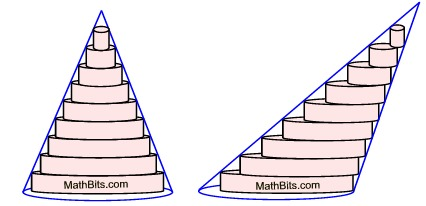
\includegraphics[width=0.85\textwidth]{images/Cavalery.jpg} 
\end{minipage}%
\hfill
\begin{minipage}{0.5\textwidth}\RaggedRight
Геометрическая идея: если взять две фигуры и на каждом сечении их площади совпадают, то совпадают и объемы.

Например из любого <<косого>> треугольника можно сделать прямоугольный треугольник и получить $S = \frac{1}{2}ah$, поэтому у пирамид и конусов формула объема $V = \frac{1}{3}Sh$.
\end{minipage}
\end{theorem}

\begin{note}
	Аналогичные рассуждения верны и для сечений второго рода.
\end{note}
\begin{proof}
    План доказательства: на $1$ шаге докажем утверждение теоремы для множеств из $\MM(\PP)$. На $2$ шаге докажем для множеств меры $0$. На $3$ шаге представим произвольное измеримое множество через множество меры нуль и множество из $\MM(\PP)$. На $4$ шаге докажем теорему для пространств $\sigma$-конечной меры.\\
    \underline{Шаг 1.} Определим $\PP = \{A \times B \mid A \in \MM, B \in \NN \}$. Предположим, что $\mu(X) < +\infty$ и $\nu(Y) < +\infty$, а $C \in \MM(\PP)$ и пока что докажем теорему для такого $C$.\\
    Пусть $\M$~---~такая система подмножеств $X \times Y$, что \begin{itemize}
        \item $\forall E \in \M \  \forall x \in X \hookrightarrow E_x \in \NN$;
        \item $x \mapsto \nu(E_x)$~---~измеримая функция.
    \end{itemize}

    Заметим следующие факты про $\MM$: \\
    1)  $\PP \subset \M $ ведь в полукольце измеримые множества, тогда сечение просто постоянная а значит измеримая функция.\\
    2) В тоже время, очевидно, что $\M$~---~симметрично, и всякое множество входит в систему со своим дополнением (в силу конечности меры $\nu(E_x^c) = \nu(Y) - \nu(E_x)$). \\
    3) Кроме того, если $C_1, C_2 \in \M$ и $C_1 \cap C_2 = \emptyset$, то $(C_1)_x \cap (C_2)_x = \emptyset$, а значит $\nu((C_1 \cup C_2)_x) = \nu((C_1 \sqcup C_2)_x) = \nu((C_1)_x) + \nu((C_2)_x)$, а следовательно $C_1 \sqcup C_2 \in \M$. \\
    Поскольку $\M \supset \PP$, и замкнуто относительно дополнения и дизъюнктного объединения, то оно содержит произвольные конечные объединения элементов полукольца (которые реализуются как дизъюнктные по соответствующей теореме). В тоже время, $X \times Y \in \PP$, а значит $\M$ содержит минимальную алгебру, порожденную этим полукольцом $\A(\PP)\subset\M $. \\
    4) $\M$ - это монотонный класс. Пусть $\{C_i\}$~---~возрастающая последовательность множеств в $\M$. Поскольку $\bigcup\limits_{n = 1}^\infty (C_n)_x = \biggl(\bigcup\limits_{n = 1}^\infty C_n\biggr)_x \in \NN$ и по непрерывности меры снизу \[x \mapsto \nu\biggl(\biggl(\bigcup\limits_{n = 1}^\infty C_n\biggr)_x\biggr) = \lim\limits_{n \rightarrow +\infty} \nu((C_n)_x).\]
    А значит $f: x \mapsto \nu(C_x)$~---~измерима как поточечный предел последовательности измеримых, следовательно $C \in \M$, т.е. $\M$~---~монотонный класс. Тогда по теореме о монотонном классе $\M \supset \MM(\PP)$, и условия 1) и 2) теоремы выполнены для всех $C \in \MM(\PP)$. \\
    Теперь проверим выполнение условия $3)$:\\ Пусть $C \in \PP$. Тогда $3)$~---~верно. Если рассматривать $\Phi: C \mapsto \int\limits_{X} \nu(C_x)d\mu(x)$ как функцию множества, то она является счётно-аддитивной мерой (интеграл неотрицательной измеримой функции~---~счетно-аддитивная функция множества). Но тогда, поскольку эта функция на $\PP$ совпадает с $\mu\otimes\nu$, то в силу единственности продолжения меры на минимальную $\sigma$-алгебру, $\Phi \equiv \mu\otimes\nu$ на $\MM(\PP)$. На данном этапе принцип Кавальери доказан для $\MM(\PP)$ \\
    \underline{Шаг 2.} Пусть теперь $C \in \MM \otimes \NN$ является измеримым множеством меры нуль. Тогда пользуясь леммой существует его <<более хороший>> envelope: $\exists \Tilde{C} \in \MM(\PP)$ т.ч. $ C \subset\Tilde{C} $ и $\mu\otimes\nu(\Tilde{C}) = 0$. Поскольку для $\Tilde{C}$ утверждения теоремы доказаны на 1 шаге, то $\forall x \in X \hookrightarrow (\Tilde{C})_x \in \NN$ и 
    $$0 = \mu\otimes\nu(\Tilde{C}) = \int\limits_X \nu(\Tilde{C}_x)d\mu(x) \Rightarrow \nu(\Tilde{C}_x) = 0 \ \mu \text{-п.в.} \ x \in X.$$
    В силу включения $C_x \subset \Tilde{C}_x$ и полноты меры $\nu$, там где мы получаем $\nu(\Tilde{C}_x)$ = 0 там и $\nu(C_x) = 0$. Тогда $C_x \in \NN, \mu$-п.в. $x \in X$. Утверждения $2)$ и $3)$ очевидны (функция, п.в. равная нулю, очевидно, измерима в широком смысле, а ноль действительно равен интегралу от равной п.в. нулю функции). \\
    \underline{Шаг 3.} Если теперь произвольное множество $C \in \MM \otimes \NN$, то $C = \Tilde{C} \setminus e$, где $\mu\otimes\nu(e) = 0$, а $\Tilde{C} \in \MM(\PP)$.\\
    Используем предыдущий шаг и получаем $\NN \ni C_x = \Tilde{C}_x \setminus e_x$~---~при $\mu$-п.в. $x \in X$. А функция $x \mapsto \nu(C_x) = \nu(\Tilde{C}_x) - \nu(e_x)$, определённая почти везде, совпадает со значениями $\nu(\Tilde{C}_x)$ при $\mu$-п.в. $x \in X$, что влечёт её измеримость в широком смысле и равенство $3)$. \\
    \underline{Шаг 4.} Теперь перейдём к $\sigma$-конечным пространствам $X$ и $Y$: $X = \bigsqcup\limits_{i = 1}^\infty X_i$ и $Y = \bigsqcup\limits_{j = 1}^\infty Y_j$. \\
    Пусть $C \in \MM \otimes \NN$. Оно разбивается на $C_{n, k} = C \cap (X_n \times Y_k)$. Для каждого из множеств $C_{n, k}$ теорема верна. Тогда очевидна справедливость $(1)$ на всём пространстве. Но, тогда \[\mu\otimes\nu(C_{n, k}) = \int\limits_{X_k}\nu(Y_n \cap C)d\mu(x).\]
    Т.к. $C_x = \bigsqcup\limits_{k = 1}^\infty (Y_k \cap C_x)$, то $\nu(C_x) = \sum\limits_{k = 1}^\infty \nu(Y_k \cap C_x)$~---~измеримая в широком смысле функция. И, наконец, используя теорему Леви, получим \[\int\limits_X \nu(C_x)d\mu(x) = \sum\limits_{n = 1}^\infty \int\limits_{X_n} \nu(C_x)d\mu(x) = \sum\limits_{n = 1}\sum\limits_{k = 1}\int\limits_{X_n}\nu(Y_k \cap C_x)d\mu(x) = \sum\limits_{n, k}\mu\otimes\nu(C_{n, k}) = \mu\otimes\nu(C).\]
\end{proof}